This chapter describes the details in the numerical implementation of the CELMA code

\section{Obtaining \texorpdfstring{$\phi$}{the potential}}
%
We observe the dependency of $\phi$ in \cref{eq:celma_dens,eq:celma_mom_dens,eq:celma_j_par,eq:celma_vortD_evolution}, but that $\phi$ is not described by a initial boundary value problem equation.
Instead, we must find alternative ways of extracting $\phi$.
We will in the following discuss two ways of doing so.
% TODO: Delete me if not in thesis
%       extra/constraint can be inserted here

\subsection{As a matrix inversion problem}
%
The problem of obtaining $\phi$ can be posed as a matrix problem $A\ve{x}=\ve{b}$, where $\ve{x}$ is an array of all the spatial values of $\phi$ ordered in some way, and $\ve{b}$ is an array of all the spatial values of $\Omega^D$ ordered in the same way.
Since we are working in an orthogonal coordinate system, we have that $\Om^D = \div\L(n\frac{\grad_\perp\phi}{B}\R) = \grad_\perp\cdot\L(n\frac{\grad_\perp\phi}{B}\R)$, as no basis vector parallel to the magnetic field can be obtained from taking the derivative of the vector $n\frac{\grad_\perp\phi}{B}$, which has only perpendicular components.
Thus, in our case, we can solve the $A\ve{x}=\ve{b}$ system for each plane perpendicular to the magnetic field.
That is, our matrix $A$ would be a $n_x \times n_y$ matrix, where $n_x$ and $n_y$ is the number of points for the two perpendicular directions
%
\footnote{
Note that in the BOUT++ implementation, $y$ is chosen as the direction parallel to the magnetic field.
This is due to historical reasons.
$n_y$ would be named $n_z$ in BOUT++ convention.
In order not to confuse readers unfamiliar with BOUT++, $z$ is chosen as the coordinate along the magnetic field unless other is specified.
}%
%
.
We note that if $\div\L(n\frac{\grad_\perp\phi}{B}\R)$ were not purely perpendicular, we would have to solve $A\ve{x}=\ve{b}$ for the whole domain.
In other words, the size of matrix $A$ would be $n_x \times n_y \times n_z$, and would be considerably harder to solve numerically.

As noted in \cite{Wiesenberger2014Phd} (in the case where $P=1$, that is, in the finite difference case), the discretization of the elliptic equation $\div\L(n\frac{\grad_\perp\phi}{B}\R)=\Om^D$ can be formulated in a symmetric manner, when special care is taken at the boundary.

Solving for the ghost-point, meaning that the ghost-point would be one of the unknown in $A\ve{x}=\ve{b}$, would break the symmetry.
Instead, one must reformulate the boundary condition in a way such that it becomes an equation for the ghost point.
The equation of the ghost point can then be substituted into the equations for the first/last inner point (the point just before the boundary) and thus effectively eliminating the ghost point from the set of equations.

To exemplify, consider a second order Dirichlet boundary condition with the boundary half between grid points for the equation $\partial_x^2 f = b$, where $f_{-1}$ denotes the value at the ghost point, $f_{\text{BC}}$ denotes the value at the boundary and $f_{1}$ denotes the value at the first inner ghost point.
The boundary condition can now be written $\frac{f_{-1}+f_{1}}{2}=f_{\text{BC}}$, and the equation for the first inner point could be written $\frac{f_{-1}+2f{1}+f_{2}}{(\Delta x)^2}=b_1$.
This would lead to the equation system
%
\begin{align*}
    A\cdot\ve{f}=&\ve{b}\\
    %
    \frac{1}{(\Delta x)^2}
    \begin{bmatrix}
        (\Delta x)^2\frac{1}{2} & (\Delta x)^2\frac{1}{2} & 0 & 0 & \ldots\\
        1                       & 2                       & 1 & 0 & \ldots\\
        0                       & 1                       & 2 & 1 & \ldots\\
        \vdots                  & \vdots              &\vdots&\vdots&\ddots\\
    \end{bmatrix}
    \cdot
    \begin{bmatrix}
        f_{-1}\\
        f_{1}\\
        f_{2}\\
        f_{3}\\
        \vdots
    \end{bmatrix}
    =&
    \begin{bmatrix}
        f_{\text{BC}}\\
        b_{1}\\
        b_{2}\\
        b_{3}\\
        \vdots
    \end{bmatrix}
\end{align*}
%
which is clearly non-symmetric.

The symmetric way to implement this would be to write $f_{-1}=2f_{\text{BC}}-f_{1}$ for the boundary condition, and substitute this into the 2nd order finite difference equation for the first inner ghost point.
This gives
%
\begin{align*}
    \frac{f_{-1}+2f{1}+f_{2}}{(\Delta x)^2}&=b_1\\
    \frac{2f_{\text{BC}}-f_{1}+2f{1}+f_{2}}{(\Delta x)^2}&=b_1\\
    \frac{f{1}+f_{2}}{(\Delta x)^2}&=b_1 - \frac{2f_{\text{BC}}}{(\Delta x)^2}
\end{align*}
%
This would give
%
\begin{align*}
    A\cdot\ve{f}=&\ve{b}\\
    %
    \frac{1}{(\Delta x)^2}
    \begin{bmatrix}
        1                       & 1                       & 0 & 0 & \ldots\\
        1                       & 2                       & 1 & 0 & \ldots\\
        0                       & 1                       & 2 & 1 & \ldots\\
        \vdots                  & \vdots              &\vdots&\vdots&\ddots\\
    \end{bmatrix}
    \cdot
    \begin{bmatrix}
        f_{1}\\
        f_{2}\\
        f_{3}\\
        \vdots
    \end{bmatrix}
    =&
    \begin{bmatrix}
        b_{1} - \frac{2f_{\text{BC}}}{(\Delta x)^2}\\
        b_{2}\\
        b_{3}\\
        \vdots
    \end{bmatrix}
\end{align*}
%
which is symmetric.
Although difficult, one can show that the non-linear elliptic equation in its symmetric form can be singular positive definite and thus be solved using the conjugate gradient method.
% FIXME: Add reference

\subsection{The Naulin solver}
%
The potential can also be found in an iterative way.
The method first used by Naulin in \cite{Naulin2008} will be presented here, and will be referred to as the Naulin solver.

The method can be used as long as
%
\begin{enumerate}[noitemsep,nolistsep]
    \item $\div\L(\frac{\grad_\perp\phi}{B}\R) = \frac{\grad_\perp^2\phi}{B}$
    \item $\grad f \cdot \grad_\perp g = \grad_\perp f \cdot \grad_\perp g$
\end{enumerate}
%
Point 1. is satisfied in our system as $B$ is constant, and because derivatives of the perpendicular basis vectors does not yield parallel components in our system.
Point 2. is satisfied as the dot product of the perpendicular basis vectors and the parallel basis vector is zero.
We then get that
%
\begin{align*}
    \Om^D =& \div\L(n\frac{\grad_\perp\phi}{B}\R)\\
    %
    =& n\div\L(\frac{\grad_\perp\phi}{B}\R) +
    \frac{\grad_\perp\phi}{B}\cdot\grad n
    \\
    %
    =& n\frac{\grad_\perp^2\phi}{B} +
    \grad n\cdot\frac{\grad_\perp\phi}{B}
    \\
    %
    =& n\frac{\grad_\perp^2\phi}{B} +
    \grad_\perp n\cdot\frac{\grad_\perp\phi}{B}
    \\
    %
    \Om^D =& n\frac{\grad_\perp^2\phi}{B} +
    \grad_\perp n\cdot\frac{\grad_\perp\phi}{B}
    \\
    %
    \frac{\Om^D}{n} =& \Om +
    \frac{1}{n}\grad_\perp n\cdot\frac{\grad_\perp\phi}{B}
    \\
    %
    \Om =& \frac{\Om^D}{n} -
    \grad_\perp \ln(n) \cdot\frac{\grad_\perp\phi}{B}
\end{align*}
%
Using square bracket superscript as iteration number, the algorithm can be stated in the following way:
%
\begin{algorithm}
\begin{enumerate}[noitemsep,nolistsep]
    \item Calculate
        $ \Om^{[i]} = \frac{\Om^D}{n} -
        \grad_\perp \ln(n) \cdot\frac{\grad_\perp\phi^{[i]}}{B}
        $
    \item Invert $\grad_\perp^2 \frac{\phi^{[i+1]}}{B} = \Om^{[i]}$ by the method
        described in \cref{app:lapInv}.
    \item Calculate
        $E_{\text{abs}, L_\infty} = \max \L|\phi^{[i]} - \phi^{[i+1]}\R|$
        and
        $E_{\text{rel}, L_\infty} = \max \L|\frac{\phi^{[i]} - \phi^{[i+1]}}{\phi^{[i]}}\R|$
    \item Check whether $E_{\text{abs}, L_\infty} > \text{Tolerance}_\text{abs}$
    \begin{itemize}[noitemsep,nolistsep]
        \item If yes: Check $E_{\text{abs}, L_\infty} > \text{Tolerance}_\text{rel}$
            \begin{itemize}[noitemsep,nolistsep]
                \item If yes: Assign $\phi^{[i+1]} \to \phi^{[i]}$, increase the
                    iteration number, throw an error if the iteration number is
                    above a predefined max iteration number, if not repeat from
                    step 1.
                \item Else, if no: Stop. Function returns
            \end{itemize}
        \item Else, if no: Stop. Function returns
    \end{itemize}
\end{enumerate}
\end{algorithm}

\subsection{The inner boundary condition for \texorpdfstring{$\phi$}{the potential}}
\label{sec:innerPhiBC}
%
As mentioned in \cref{sec:BCs} there are no real inner boundary in the cylinder.
However, the inversion method described in \cref{app:lapInv} requires a boundary condition for the inner $\rho$ for each mode number.
A method to do this, first used in \cite{Naulin2008} sets the inner ghost point depending on the evenness of the mode.

If the mode is even, the mode under consideration would have the same value diametrically opposite of the innermost point.
Hence, the ghost point for the inner $\rho$ value is set to the same as the value at the innermost $\rho$.

If the mode is odd, the mode under consideration would have value of the point diametrically opposite of the innermost point, but with a changed sign.
Thus, the ghost point for the inner $\rho$ value is set to the negative of the value at the innermost $\rho$.
This is depicted in \cref{fig:BCLaplace}
%
\begin{figure}[h!]
    \centering
    \begin{subfigure}[t]{0.5\textwidth}
        \centering
        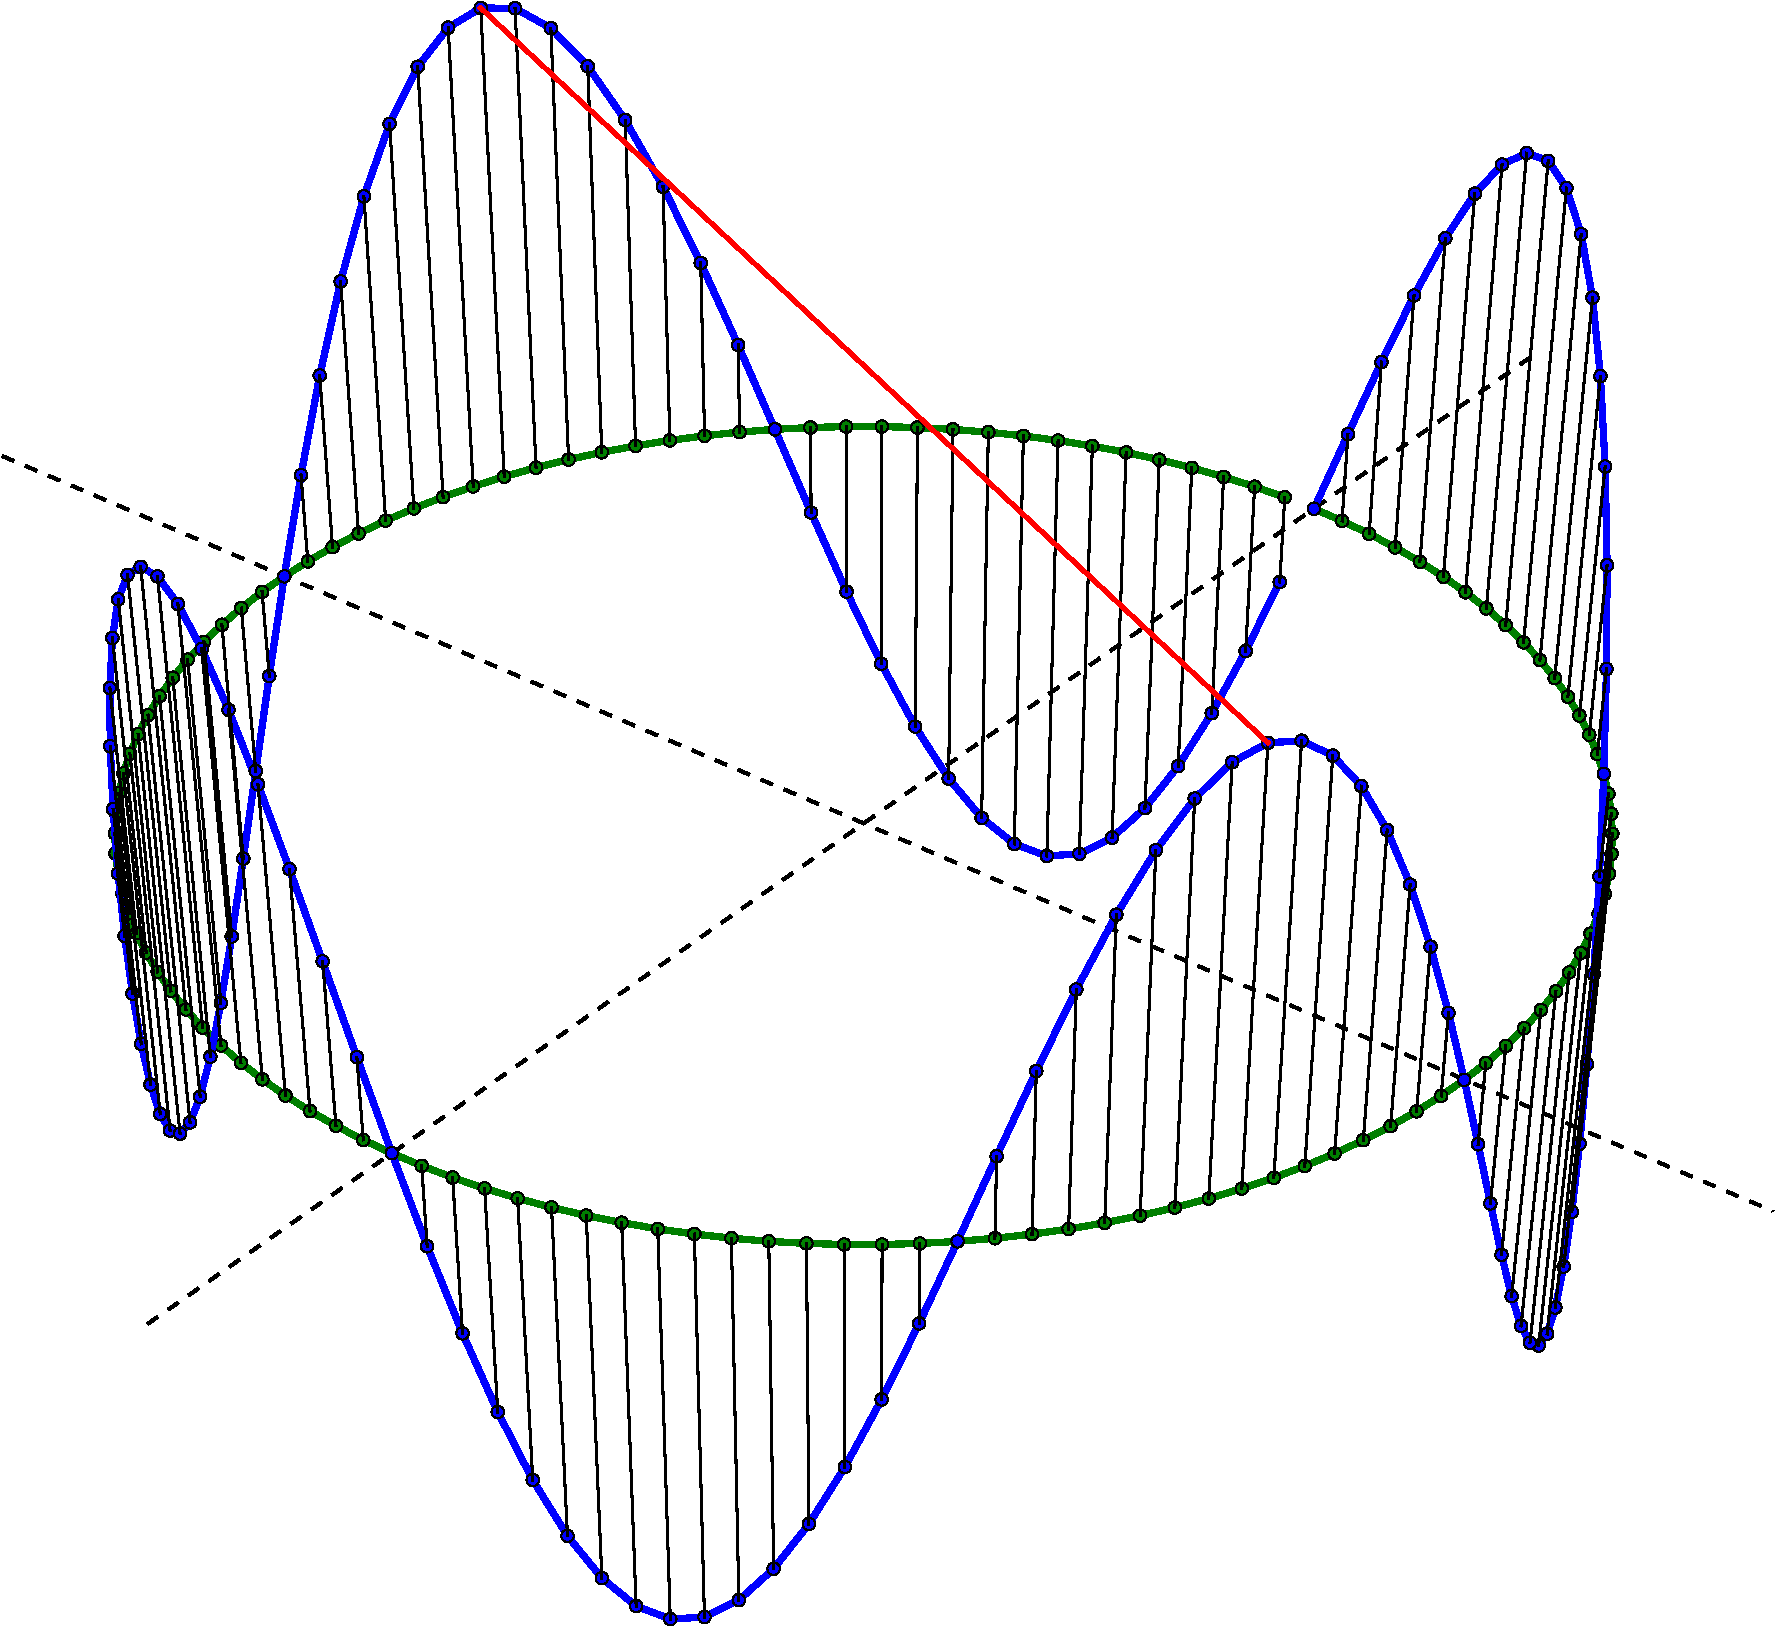
\includegraphics[width=1.0\textwidth]{fig/mode_4}
        \caption{An even mode.}
    \end{subfigure}%
    \hfill
    \begin{subfigure}[t]{0.5\textwidth}
        \centering
        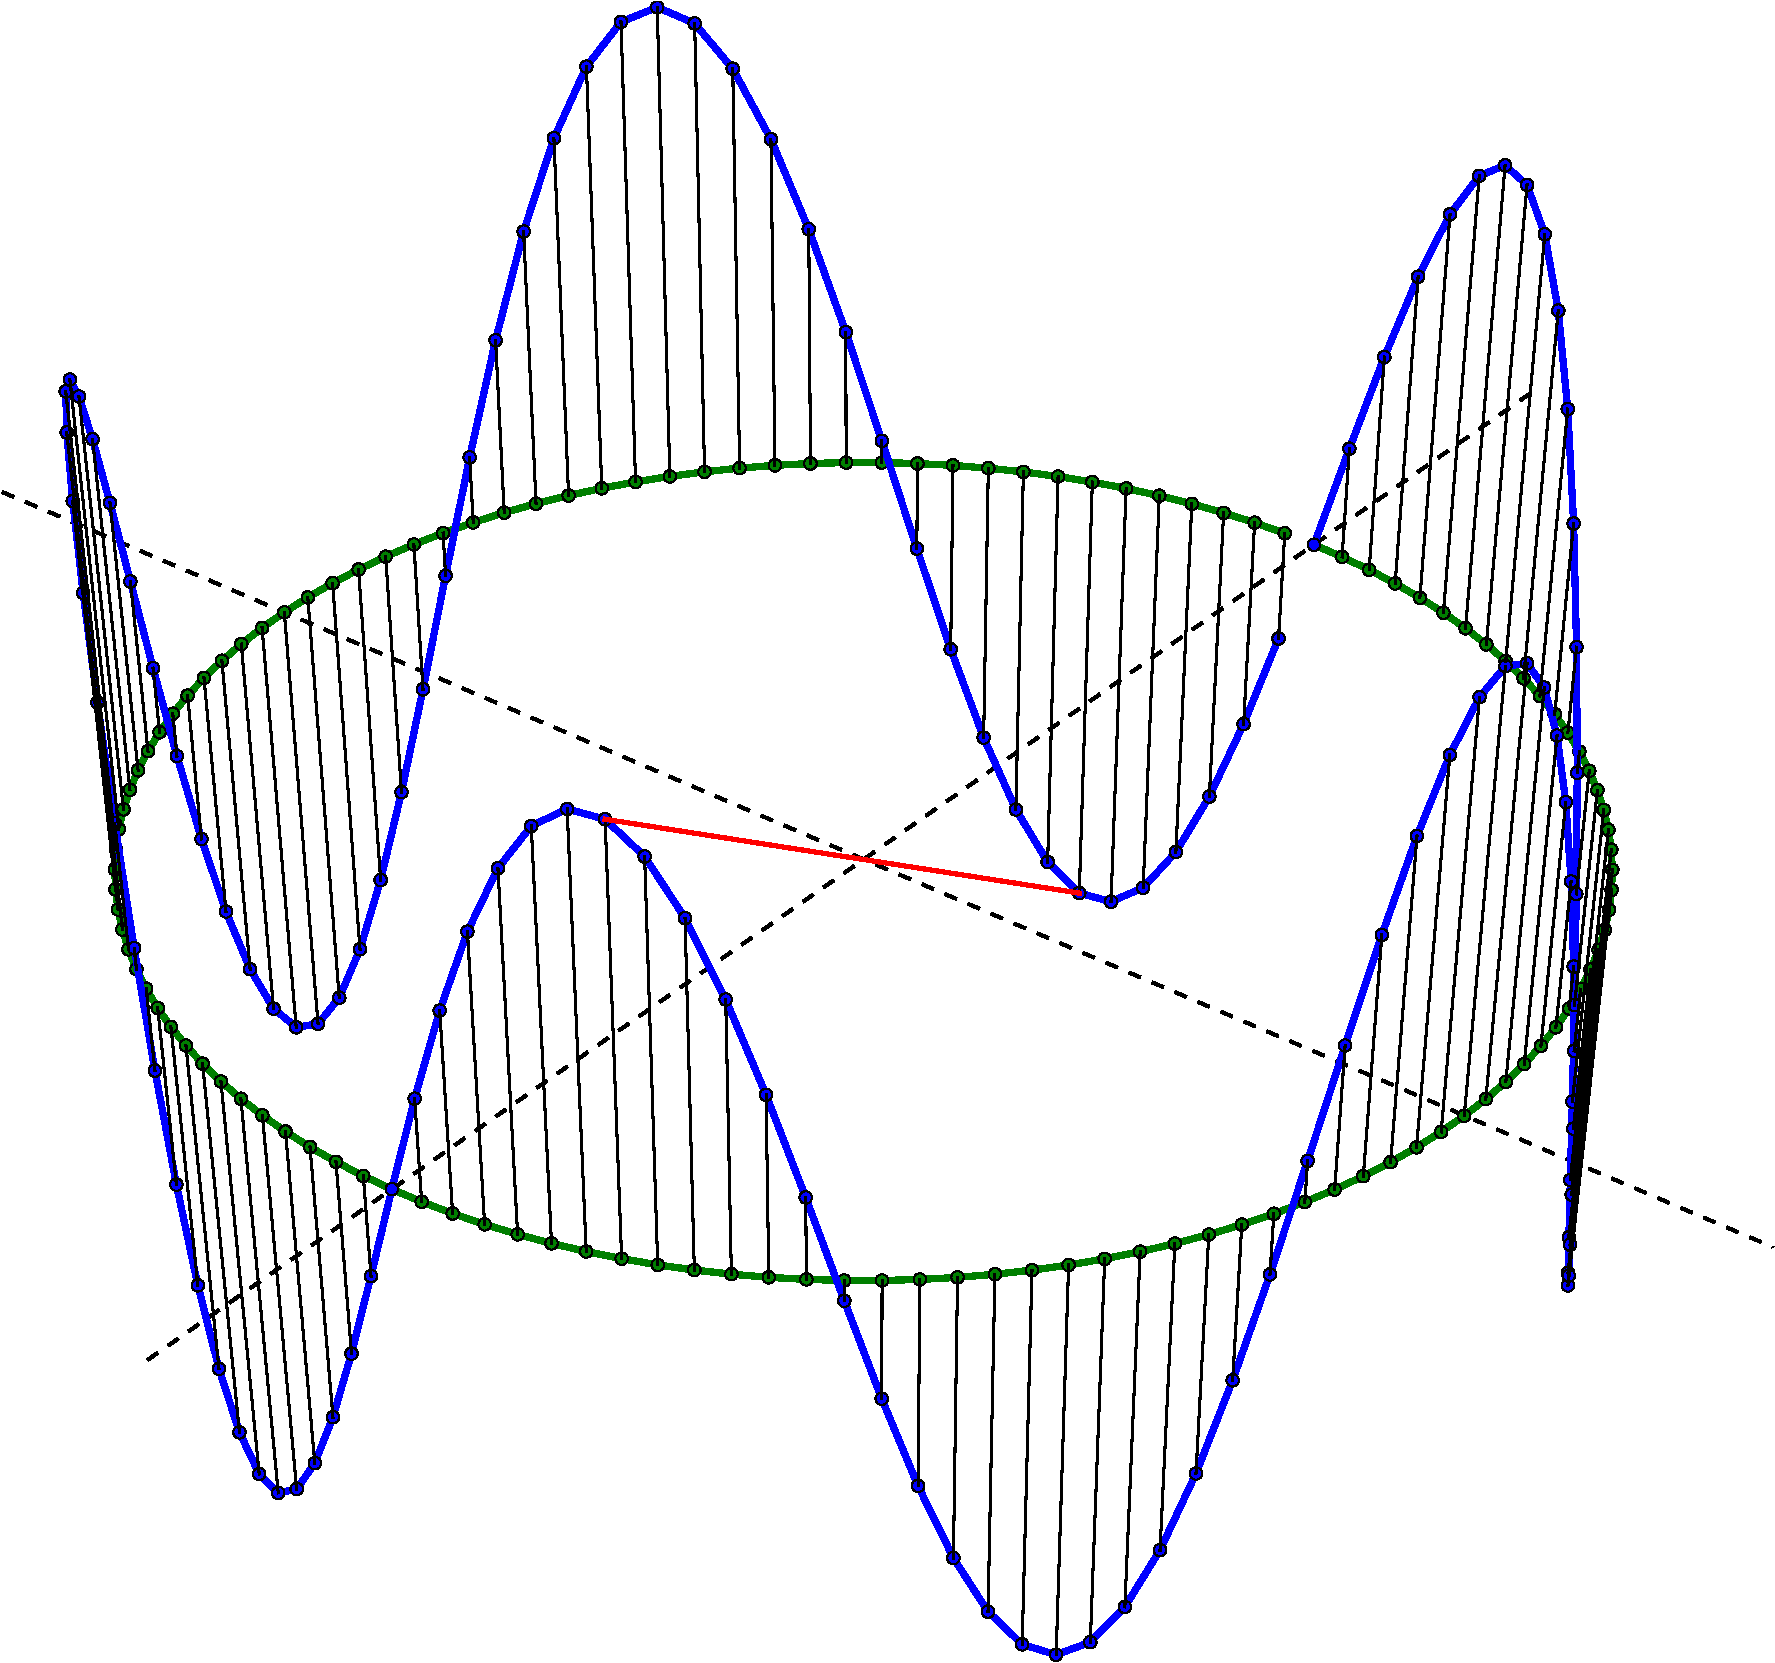
\includegraphics[width=1.0\textwidth]{fig/mode_5}
        \caption{An odd mode.}
    \end{subfigure}
        \caption{The point diametrically opposite for a mode located at radius $\rho$ has the same value as the point under consideration for an even mode, but the same value with a changed sign for even modes.
        The red soid line connects points diametrically opposite of each other.}
    \label{fig:BCLaplace}
\end{figure}



\section{Advective terms}
\label{sec:ExBadv}
%
As already noted in \cref{sec:vecAdvTerm}, we can write $\ve{E}\times\ve{B}$-advective terms as Poisson brackets.
The proof is found in \cref{app:poisson}.
The benefits of writing terms on Poisson brackets are presented in Arakawa's paper from 1966 \cite{Arakwa1966}.
In short, the paper shows that a na\"ive finite difference discretization of the Poisson bracket does not conserve energy and enstrophy, and gives an alternative way of discretize in orthogonal curvilinear coordinates in order to keep these quantities conserved.
If the energy and enstrophy is not conserved, fake generation of these quantities occur, which eventually will lead to a blow up of the simulation (in a way described by Phillips in \cite{Phillips1959}).

It is also possible to discretize the term $\{\ve{u}_E^2, n\}$ using Arakawa's method.
We observe that in cylindrical coordinates, we have
%
\begin{align*}
    \{\ve{u}_E^2, n\} &= \L\{\L(\frac{\grad_\perp \phi}{B}\R)^2, n\R\}
    \note{Constant $B$}
    \\
    %
    &= \L(\frac{1}{B}\R)^2
    \L\{\L(\L[\ve{e}^{\rho}\partial_{\rho} + \ve{e}^{\theta}\partial_{\theta}\R] \phi\R)
        \cdot
        \L(\L[\ve{e}^{\rho}\partial_{\rho} + \ve{e}^{\theta}\partial_{\theta}\R] \phi\R)
        , n\R\}
    \note{Orthogonality}
    \\
    %
    &= \L(\frac{1}{B}\R)^2
    \L\{g^{\rho\rho}\L(\partial_{\rho} \phi\R)^2+
        g^{\theta\theta}\L(\partial_{\theta} \phi\R)^2
        , n\R\}
    \\
    %
    &= \L(\frac{1}{B}\R)^2
    \L\{\L(\partial_{\rho} \phi\R)^2+ \frac{1}{\rho^2}\L(\partial_{\theta} \phi\R)^2
        , n\R\}
\end{align*}
%
Here, we must take care when we treat the ghost points.
No ghost points is needed in the $\theta$ direction, as this direction is periodic.
Thus, for $\partial_{\theta} \phi$, we only need to make sure that we take the $\theta$ derivatives at the ghost points in $\rho$.

For $\partial_{\rho} \phi$, we must re-apply the values in the $\rho$ ghost points as the derivative is not calculated there.
For the inner ghost point, the same procedure as used in
% FIXME: Add section
can be used.
For the outer ghost point, we use a fourth order Newton polynomial of the four previous points in the $\rho$ direction, evaluated in the ghost point.
If we say that $f=\partial_{\rho} \phi$, this extrapolation reads
%
\begin{align*}
    f_{0} = 4f_{-1} - 6f_{-2} + 4f_{-3} - f_{-4}
\end{align*}
%
where $f_{0}$ is the value of $f$ at the position of the ghost point and $f_{-i}$ is the value of $f$ in a position $-i\Delta \rho$ away from the ghost point (where $\Delta \rho$ is the grid spacing in $\rho$).

This way of discretizing is second order accurate, as indicated in appendix
%FIXME: Add to appendix MES
%FIXME: Add to appendix MES
%FIXME: ADD HOW PARALLEL DERIVATIVE OF RHO IS IMPLEMENTED
YOU ARE HERE




THIS IS FROM DELETED STUFF
Secondly we have
%
\begin{align*}
    u_{i,\|}\partial_\|\L(\frac{\grad_\perp \phi}{B}n\R)
    =&
    u_{i,\|}\partial_\|
    \L( \ve{e}^\rho\frac{\partial_\rho \phi}{B}n
    + \ve{e}^\theta\frac{\partial_\theta \phi}{B}n \R)
    \note{$\partial_z \ve{e}^i=0$}
    \\
    =&
    \ve{e}^\rho u_{i,\|}\partial_\|\L( \frac{\partial_\rho \phi}{B}n \R)
    + \ve{e}^\theta u_{i,\|}\partial_\|\L( \frac{\partial_\theta \phi}{B}n\R)
    \numberthis
    \label{eq:par_vec_adv_expanded}
\end{align*}
%
where we have to set the $z$ boundaries of $\frac{\partial_\rho \phi}{B}n$ and $\frac{\partial_\theta \phi}{B}n$ in order to calculate the parallel derivatives of \cref{eq:par_vec_adv_expanded} using a FDA.

\section{Artificial viscosity}\label{sec:art_visc}
%
In the derivation we have neglected terms which is of order lower than first order, as these terms are believed to have negligible contribution on the overall set of equation.
One of the drawbacks is, however, that we also have neglected viscous terms which will dampen small scales in the system.
Thus, if we no not re-introduce some dissipation for numerical purposes, energy is going to build-up on small scales, and would in the end make the simulation crash.
%FIXME: Add cite to Phillips instability if applicable

Therefore, we add a dissipation on the form
%
\begin{align*}
    D_{f, \|, \text{art}} \nabla_{\|}^2 f
    + D_{f, \perp, \text{art}} \grad_\perp^2 f
    &=
    D_{f, \|, \text{art}} \div \L(\ve{b}\ve{b}\cdot\grad\R) f
    + D_{f, \perp, \text{art}} \grad_\perp^2 f
    \note{$\partial_i \ve{b} = 0$}
    \\
    %
    &=
    D_{f, \|, \text{art}} \ve{b}\cdot\grad \L(\ve{b}\cdot\grad\R) f
    + D_{f, \perp, \text{art}} \grad_\perp^2 f
    \\
    %
    &=
    D_{f, \|, \text{art}} \partial_\|^2 f
    + D_{f, \perp, \text{art}} \grad_\perp^2 f
    \numberthis
    \label{eq:art_vort}
\end{align*}
%
by exchanging $\div \te{\pi}$ in equarion (\ref{fluideq:mom}) with \cref{eq:art_vort}.
This is a somewhat crude approximation, but serves as a good first approximation.
In the non-normalized set of equations the $D$ coefficients would have the units of dynamical viscosity, and would be normalized by
\\
%
\begin{minipage}{0.4\textwidth}
\begin{empheq}[box={\tcbhighmath[colback=yellow!5!white]}]{align*}
    &    D_{f, \text{art}}  = \wt{D}_{f, \text{art}}m_\a n_0 \rho_s c_s&
\end{empheq}
\end{minipage}
\hfill
\begin{minipage}{0.4\textwidth}
\begin{empheq}[box={\tcbhighmath[colback=yellow!5!white]}]{align*}
    &\wt{D}_{f, \text{art}}  =  \frac{D_{f, \text{art}}}{m_\a n_0 \rho_s c_s}&
\end{empheq}
\end{minipage}
\vspace{0.5cm}
\\
%
We notice that when using equation (\ref{fluideq:mom}) in the derivations, division by $n$ on the RHS of the equations occurs in the density equation and the parallel momentum equations, but not in the vorticity equation.
The artificial viscosity in the density is not divided by $n$ as $\frac{1}{n}\grad n = \ln(n)$.

\section{Time solver}
This chapter will briefly discuss the time solver used in this thesis.
At the time of writing the following time solvers are available in the BOUT++ framework
% FIXME: Mention time solvers, and add references.

The \texttt{cvode}\cite{Hindmarsh2012book} has been found to be a robust and fast time solver for solving \cref{eq:celma_dens,eq:celma_mom_dens,eq:celma_j_par,eq:celma_vortD_evolution} in time.

As \cref{eq:celma_dens,eq:celma_mom_dens,eq:celma_j_par,eq:celma_vortD_evolution} contains no mixed temporal and spatial derivatives in the equations, the PDEs can first be discretized in the spatial dimension while keeping the time derivatives continuous.
The set of PDEs is thereby rewritten to a set of ODEs (one for each of the discretized point in space) which needs to be solved simultaneously.
This method is known as the "Method of Lines" (MOL) \cite{Leveque2007book}, and is widely used when solving a set of non-linear PDEs.

The problem can now be stated in the following way:
Let $\ve{f} = \{\ln(n), nu_{i,\|}, j_\|, \Om^D\}$, for $\ln(n)$, $nu_{i,\|}$, $j_\|$ and $\Om^D$ discretized in space.
That is, $\ve{f}$ is the tuple of the time dependent variables, and contains $\ln(n)_{0,0,0}$, $\ln(n)_{0,0,1}$ \ldots $\ln(n)_{n_\rho,n_z,n_\theta}$, \ldots $nu_{{i,\|}_{0,0,0}}$, \ldots $\Om^D_{n_\rho,n_z,n_\theta}$ where the subscripts denotes the grid index.
Hence, we would like to solve
%
\begin{align}
    \parti{\ve{f}(t)}{t} = F(\ve{f})
    \label{eq:MOL}
\end{align}
%
for $\ve{f}$, where $F(\cdot)$ denotes the nonlinear operator which contains discretized differential operators in the spatial dimension.

\cref{eq:MOL} can be stepped forward in time by using an appropriate time solver, like Runge-Kutta or a Linear Multistep Method (LMM).
Due to it's good stability properties \cite{Leveque2007book} an implicit LMM has been chosen.
By using a generic LMM to \cref{eq:MOL}, we get
%
\begin{align*}
    \sum_{j=0}^{r}\a_j\ve{f}(t_{n+j}) =& k\sum_{j=0}^{r}\b_jF(\ve{f}(t_{n+j}), t_{n+j})\\
    %
    \a_r\ve{f}(t_{n+r}) + \sum_{j=0}^{r-1}\a_j\ve{f}(t_{n+j}) =&
    \b_rF(\ve{f}(t_{n+r}), t_{n+r}) +
    k\sum_{j=0}^{r-1}\b_jF(\ve{f}(t_{n+j}), t_{n+j})\\
    %
    \ve{f}(t_{n+r})
    -
    \frac{\b_r}{\a_r}F(\ve{f}(t_{n+r}), t_{n+r})
    =&
    \frac{k}{\a_r}\sum_{j=0}^{r-1}\b_jF(\ve{f}(t_{n+j}), t_{n+j})
    - \frac{1}{\a_r}\sum_{j=0}^{r-1}\a_j\ve{f}(t_{n+j})
    \numberthis
    \label{eq:LMM}
\end{align*}
%
The method is implicit if $\b_r\neq0$.
That is, the solution for the next time step depends on the next time step itself.
In other words \cref{eq:LMM} can be stated as an optimization problem.
By defing $\frac{\b_r}{\a_r}\defined\gamma$, we have
%
\begin{align*}
    \ve{f}(t_{n+r})
    - \gamma F(\ve{f}(t_{n+r}), t_{n+r})
    - \frac{k}{\a_r}\sum_{j=0}^{r-1}\b_jF(\ve{f}(t_{n+j}), t_{n+j})
    + \frac{1}{\a_r}\sum_{j=0}^{r-1}\a_j\ve{f}(t_{n+j})
    =
    G(\ve{f}(t_{n+r}))
    =&
    0
\end{align*}
%
Which we would like to solve for $\ve{f}(t_{n+r})$.
This can be done by using Newton Raphson's method.
I. e. we do a multivariate Taylor expansion of $G(\ve{f}(t_{n+r}))$ around an approximate point $\ve{f}_l(t_{n+r})$, and retain only the linear terms
%
\begin{align*}
    G(\ve{f}(t_{n+r})) \simeq
    G(\ve{f}_{l}(t_{n+r})) + \L(\parti{ G(\ve{f}_{l}(t_{n+r})) }{\ve{f}_{l}(t_{n+r})}\R)
    \L(\ve{f}(t_{n+r}) - \ve{f}_{l}(t_{n+r})\R)
\end{align*}
%
as $ G(\ve{f}(t_{n+r})) = 0$, we get
%
\begin{align*}
    0 \simeq
    G(\ve{f}_{l}(t_{n+r})) + \L(\parti{ G(\ve{f}_{l}(t_{n+r})) }{\ve{f}_{l}(t_{n+r})}\R)
    \L(\ve{f}(t_{n+r}) - \ve{f}_{l}(t_{n+r})\R)
\end{align*}
%
the solution $\ve{f}(t_{n+r})$ to this problem can then serve as the next iteration, so that
%
\begin{align*}
    \ve{f}_0(t_{n+r}) =& \ve{f}(t_{n+r-1})\\
    \ve{f}_{l+1}(t_{n+r}) =& \ve{f}_l(t_{n+r})-
    \L(\parti{ G(\ve{f}_{l}(t_{n+r})) }{\ve{f}_{l}(t_{n+r})}\R)^{-1}
    G(\ve{f}_{l}(t_{n+r})),
\end{align*}
%
where $l$ denote the $l$'th Newton iteration.
The iterations can be rewritten to
%
\begin{align}
    \parti{ G(\ve{f}_{l}(t_{n+r})) }{\ve{f}_{l}(t_{n+r})}
    \L( \ve{f}_{l+1}(t_{n+r}) - \ve{f}_l(t_{n+r}) \R)
    =&
    -G(\ve{f}_{l}(t_{n+r}))
    \label{eq:newtonIt}
\end{align}
%
Where
%
\begin{align*}
    \parti{ G(\ve{f}(t_{n+r})) }{\ve{f}(t_{n+r})}
    =&
    \parti{ }{\ve{f}(t_{n+r})}
    \L(
    \ve{f}(t_{n+r})
    - \gamma F(\ve{f}(t_{n+r}), t_{n+r})
    - \frac{k}{\a_r}\sum_{j=0}^{r-1}\b_jF(\ve{f}(t_{n+j}), t_{n+j})
    + \frac{1}{\a_r}\sum_{j=0}^{r-1}\a_j\ve{f}(t_{n+j})
    \R)
    \\
    =&
    \mathbb{I}
    - \gamma\parti{F(\ve{f}(t_{n+r}), t_{n+r})}{\ve{f}(t_{n+r})}
    \\
    =&
    \mathbb{I} - \gamma\mathbb{J}
    \numberthis
    \label{eq:AInNewton}
\end{align*}
%
By inserting \cref{eq:AInNewton} in \cref{eq:newtonIt}, we get
%
\begin{align*}
    \L( \mathbb{I} - \gamma\mathbb{J}\R)
    \L( \ve{f}_{l+1}(t_{n+r}) - \ve{f}_l(t_{n+r}) \R)
    =&
    -G(\ve{f}_{l}(t_{n+r}))
\end{align*}
%
which can be recast to
%
\begin{align}
    A \ve{x} =& \ve{b}
    \label{eq:newtonInverse}
\end{align}
%
In other words, we need to invert $A$ (that is $\L( \mathbb{I} - \gamma\mathbb{J}\R)$) for each Newton iteration.
As the system of equations in \cref{eq:newtonInverse} is rather large (and also generally non-symmetric), a robust an fast method is sougth to solve for $\ve{x}$.
This can be done by using the \textbf{G}eneralized \textbf{M}inimal \textbf{RES}idual method (GMRES).

% NOTE: Finding the Krylov subspace is almost like using the von Mises (power iteration method) of finding the eigenvector with the highest eigenmode
This method approximates the exact solution of \cref{eq:newtonInverse} by a vector in the Krylov subspace (spanned by vectors obtained through the Arnoldi process), which minimizes the residual $\ve{r}_n = A \ve{x}_n - \ve{b}$. See \cite{Saad2003book} for details.

One of the advantages is that the Jacobian for the GMRES needs not to be expanded in memory as the Arnoldi process only needs to evaluate a Jacobian vector product \cite{Knoll2004}.

The method is also easily preconditioned%
\footnote{
    To precondition means to find a $P_L$ and/or $P_R$, which is easy to invert, and makes either $(P_L^{-1}A) \ve{x} = P_L^{-1}\ve{b}$, $(A P_R^{-1})P_R\ve{x} = \ve{b}$ or $(P_L^{-1}AP_R^{-1}) \ve{x} = P_L^{-1}\ve{b}$ numerically easier to solve than \cref{eq:newtonInverse}, as the matrices in parantheses is used in finding vectors spanning the Krylov subspace rather than $A$ itself.
}
%
, as shown in \cite{Dudson2012}.
Although preconditioning is expected to give substaintial speed-ups \cite{Hindmarsh2012book}, it is outside the scope of this thesis.

% FIXME: Mention that IMEX has been tried out, but has not worked
